\newpage
\newpage
%\pagestyle{standardpagestyle}
%\thispagestyle{empty}
\section{Evaluation}
In this section, we evaluate LittlePanorama to answer the following four questions: (1) How efficient is LittleParorama? (2) Can LittlePanorama detect crash failures? (3) Can LittlePanorama detect gray failures? (4) Can LittlePanorama handle transient failures properly?

We evaluate LittlePanorama on failures caused by 4 bugs listed in Table ~\ref{tab:failures}. The two bugs that crash leaders/followers are introduced artificially for the purpose of demonstration. The other two that result in gray failures are bugs found in production and used in the original paper. We evaluate these bugs in an ideal way --- triggering them manually instead of simulating a production workflow. The main constraint that limits us from evaluating LittlePanorama on more bugs or in a more complex setting is the time and effort needed. We pick bugs that are representative and easy to reproduce and test.

\begin{table}[!tb]
\begin{tabular}{p{0.24\columnwidth}p{0.60\columnwidth}p{0.06\columnwidth}}%{l|l|l}

\toprule
\textbf{BugId} & \textbf{Description} & \textbf{Gray} \\
\midrule
  artificial-01   &    An artificially injected bug that causes the leader to fail  &  No  \\
 artificial-02      &   An artificially injected bug that causes the follower to fail  &  No  \\  
zookeeper-2201      &   Zookeeper service becomes unavailable due to transient network partition &  Yes \\
zookeeper-2247      &   Zookeeper service becomes unavailable when leader fails to write transaction log &  Yes \\
\bottomrule
\end{tabular}
\vspace{0.5em}
\caption{Bugs used in our experiments. Gray indicates whether the resultant failure is a gray failure or not.}
\label{tab:failures}
\end{table}


\subsection{Experiment Setup}
We use the VM provided to run all the experiments. This VM has a single-core 2.4 GHz Intel Xeon E5-2676 CPU, 1 GB of RAM and a 7.7 GB HVM disk. It runs Ubuntu 18.04 LTS (Bionic Beaver). We also modify the source code of Zookeeper version 3.4.6 to introduce hooks and artificial bugs. We evaluate LittlePanorama with a three-node Zookeeper ensemble listening on different ports.

\subsection{Performance}
\subsubsection{Reporting Speed} Table ~\ref{tab:microbench} shows the average latency of reporting an observation in LittlePanorama and Panorama respectively. Two things can be observed here. First, reporting an observation is cheap, as the average latency is less than 1 ms. This is because reporting an observation only incurs a local RPC. Second, LittlePanorama is about 3x faster than Panorama in terms of reporting speed. We attribute LittlePanorama's performance gain to the fact that it implements a much simpler datastructure and saves everything in memory.

\begin{table}[!tb]
\begin{tabular}{p{0.24\columnwidth}p{0.33\columnwidth}p{0.33\columnwidth}}%{l|l|l}

\textbf{Operation} & \textbf{Panorama} & \textbf{LittlePanorama} \\
\midrule
  Report   &    753 $\mu$s  &  194 $\mu$s  \\
\end{tabular}
\vspace{0.5em}
\caption{Average speed of reporting an observation (Report)}
\label{tab:microbench}
\end{table}

\subsubsection{Judging Speed\label{subsubsec:js}} Figure ~\ref{fig:judge} plots the average judging speed of LittlePanorama and Panorama with varying number of observations. LittlePanorama's performance degrades as the number of observations increases, as in the worst case it would examine all observations. However, Panorama does not have this problem. After a close inspection of Panorama's source code, we realize that this performance stability is due to the fact that Panorama only considers the two most recent observations. The original paper refers to this behavior as \textit{bounded-look-back}.

\begin{figure}[!tb]
\centering
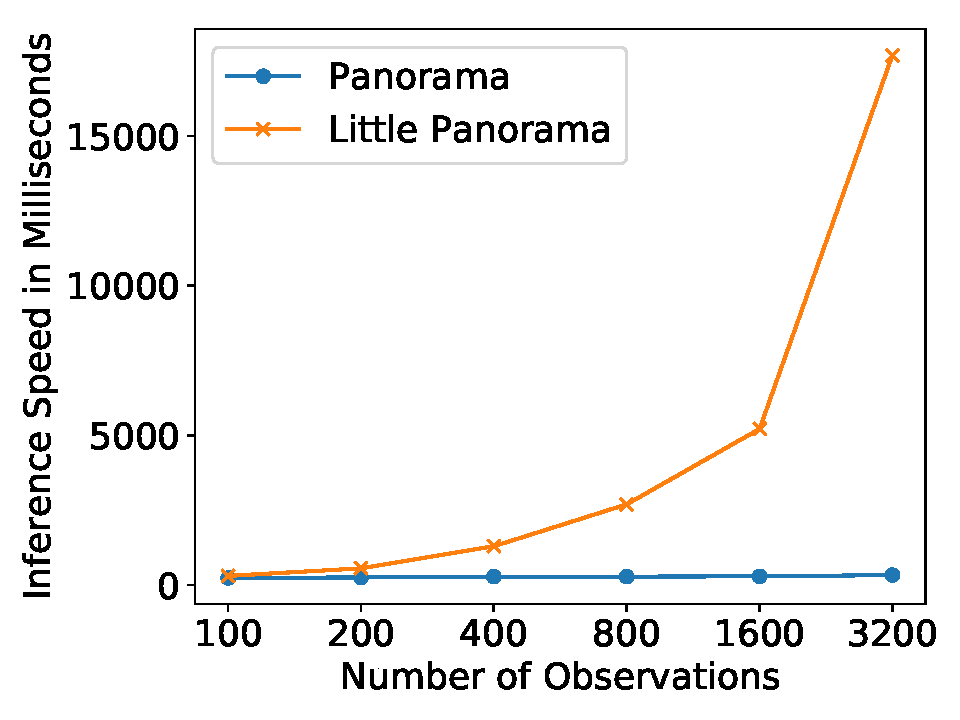
\includegraphics[scale=0.4]{figs/inference.pdf}
\vspace{-1em}
\caption{Judging Speed
\label{fig:judge}
}
\end{figure}

\subsubsection{Propagation Speed} Figure ~\ref{fig:propagation} graphs the average delay of propagating one observation to all peers with various peer sizes. The propagation delay in both cases is proportional to the number of peers, matching what is reported in the original paper. However, looking at Panorama's source code, it seems that the authors have parallelized the process of propagation, which in theory should give a better performance. Unfortunately, we fail to observe any improvement. Our benchmark code is carefully examined such that the probability of this phenomenon caused by a bug in our code is low. Another possible explanation is that the CPU used in our experiments only has one core, burying the performance gain of thread-level parallelism.

\begin{figure}[!tb]
\centering
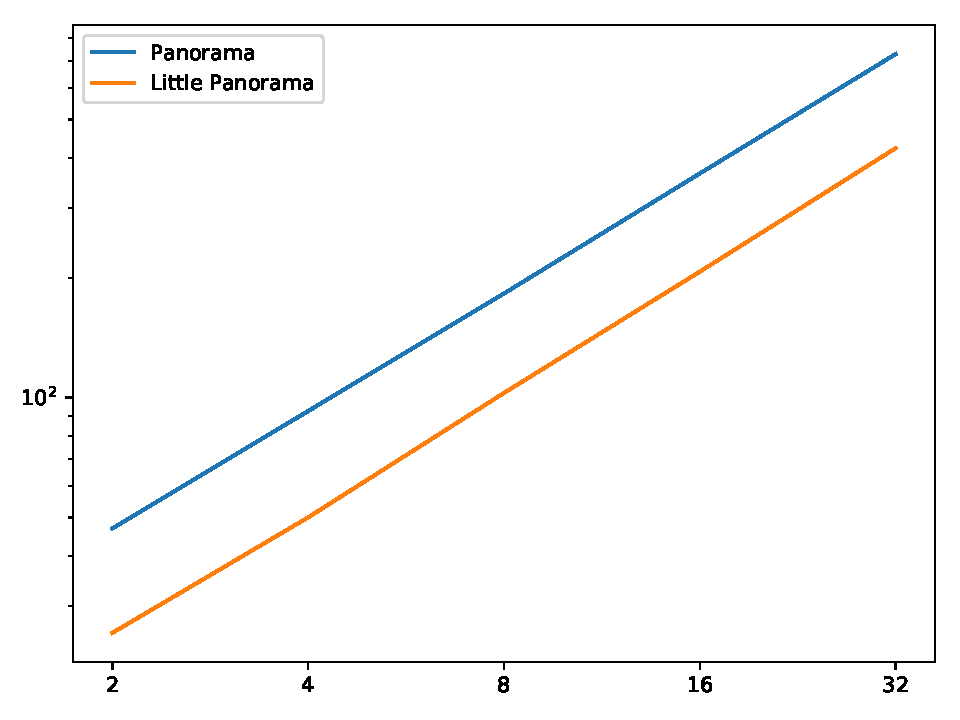
\includegraphics[scale=0.4]{figs/propagation.pdf}
\vspace{-1em}
\caption{Propagation Speed
\label{fig:propagation}
}
\end{figure}

\subsection{Detection of Crash Failures}
Both Panorama and LittlePanorama are designed to detect complex real-world failures. Detecting simple crash failures can serve as a sanity check on the capability of both systems. We inject two crash failures bugs --- artificial-01 and artificial-02, which will crash leader and follower respectively when triggered. Table ~\ref{tab:crashperf} shows the detection time. We see that it takes less than 200 ms to detect both failures, matching the results ($\sim$10 ms) reported in the original paper. Further, we observe little difference in performance between LittlePanorama and Panorama.

\begin{table}[!tb]
\begin{tabular}{p{0.24\columnwidth}p{0.33\columnwidth}p{0.33\columnwidth}}%{l|l|l}

\toprule
 & \textbf{Panorama} & \textbf{LittlePanorama} \\
\midrule
  artificial-01    &    128 ms  &  138 ms  \\
  artificial-02       &   81 ms   &  45 ms \\
\bottomrule
\end{tabular}
\vspace{0.5em}
\caption{Detection time for crash failures}
\label{tab:crashperf}
\end{table}

\subsection{Detection time for gray failures}
Being able to detect complex gray failures is one of the keys goals. To evaluate both systems' ability to detect gray failures, we reuse two gray failures from the original paper. They are real-world production failures found in ZooKeeper. Both of them would cause the ZooKeeper service to be temporarily unavailable but not crashing any ZooKeeper server. Table ~\ref{tab:grayperf} shows detection time. The detection times have a minimum of 0.2 s and a maximum of 7 s. We 

\begin{table}[!tb]
\begin{tabular}{p{0.24\columnwidth}p{0.33\columnwidth}p{0.33\columnwidth}}%{l|l|l}

\toprule
 & \textbf{Panorama} & \textbf{LittlePanorama} \\
\midrule
  zookeeper-2201    &   66850 ms   &  67038 ms \\
  zookeeper-2247    &   2632 ms    &  2195 ms  \\
\bottomrule
\end{tabular}
\vspace{0.5em}
\caption{Detection time for gray failures}
\label{tab:grayperf}
\end{table}

\subsection{Transient Failure, Normal Operations}
blahblah Figure ~\ref{fig:transient}.

\begin{figure}[!tb]
\centering
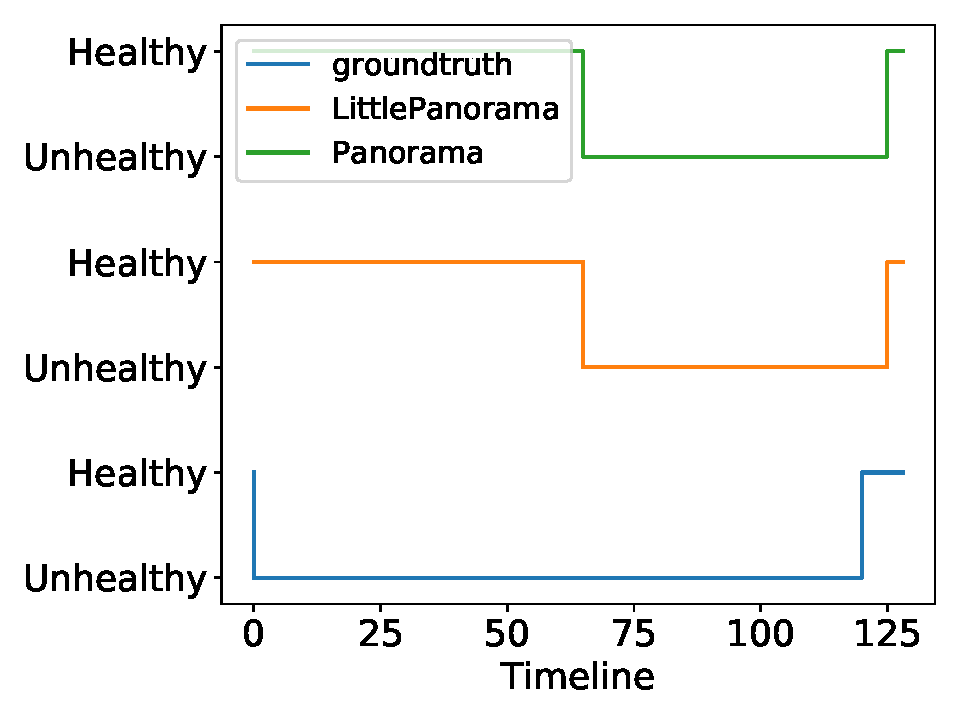
\includegraphics[scale=0.4]{figs/transient.pdf}
\vspace{-1em}
\caption{Transient Failure
\label{fig:transient}
}
\end{figure}

%%%
% Creating Testing Environment For Leader Failure
% Time To Detect Leader Failure: 128 ms

% Creating Testing Environment For Follower Failure
% Time To Detect Follower Failure: 81 ms

% Creating Testing Environment For Gray Failure 1
% Setting up nodes
% Setting up regular connections from clients
% Triggering gray 1
% Time To Detect Gray Failure 1: 66850 ms

% Creating Testing Environment For Gray Failure 2
% Triggering gray 2
% Time To Detect Gray Failure 2: 2632 ms

% Creating Testing Environment For Coming Back
% Setting up nodes
% Setting up regular connections from clients
% Triggering gray 1
% Time To Detect Failure: 66881 ms
% Start Pulling Again From Clients
% Time To Detect Revival: 125774 ms


%%% 
% Creating Testing Environment For Leader Failure
% Time To Detect Leader Failure: 138 ms

% Creating Testing Environment For Follower Failure
% Time To Detect Follower Failure: 45 ms

% Creating Testing Environment For Gray Failure 1
% Setting up nodes
% Setting up regular connections from clients
% Triggering gray 1
% Time To Detect Gray Failure 1: 67038 ms

% Creating Testing Environment For Gray Failure 2
% Triggering gray 2
% Time To Detect Gray Failure 2: 2195 ms

% Creating Testing Environment For Coming Back
% Setting up nodes
% Setting up regular connections from clients
% Triggering gray 1
% Time To Detect Failure: 66584 ms
% Start Pulling Again From Clients
% Time To Detect Revival: 125607 ms
